\documentclass[10pt]{extarticle}
\usepackage[margin=1.5cm]{geometry}
\usepackage[UKenglish]{babel}
\usepackage{amssymb}
\usepackage{amsmath}
\usepackage{bm}
\usepackage{graphicx}
\graphicspath{{./pics/}}
\usepackage{physics}

%% vectors and matrices
\renewcommand{\v}[1]{{\bm #1}}
\renewcommand{\dv}[1]{\dot{\bm{#1}}}
\newcommand{\ddv}[1]{\ddot{\bm{#1}}}
\newcommand{\hv}[1]{\hat{\bm{#1}}}
\newcommand{\m}[1]{[ #1 ]}
\renewcommand{\t}[1]{\widetilde{\bm{#1}}}
\newcommand{\bfit}[1]{\textbf{\textit{#1}}}

%% differential and integral operators
\renewcommand{\d}{\text{d}}
\renewcommand{\dd}[2]{\frac{\d #1}{\d #2}}
\newcommand{\ddd}[2]{\frac{\d^2 #1}{\d #2^2}}
\newcommand{\ddt}[1]{\frac{\d #1}{\d t}}
\newcommand{\dddt}[1]{\frac{\d^2 #1}{\d t^2}}
\newcommand{\pd}[2]{\frac{\partial #1}{\partial #2}}
\newcommand{\pdd}[2]{\frac{\partial^2 #1}{\partial #2^2}}
\renewcommand{\grad}{\boldsymbol \nabla}
\renewcommand{\div}{\boldsymbol \nabla \cdot}
\renewcommand{\curl}{\boldsymbol \nabla \times}
\newcommand{\lap}{\nabla^2}

%% constants
\newcommand{\eo}{\epsilon_0}

%% statistics
\newcommand{\E}{\text{E}}
\newcommand{\Var}{\text{Var}}
\newcommand{\SD}{\text{SD}}
\newcommand{\SE}{\text{SE}}
\newcommand{\Cov}{\text{Cov}}
\newcommand{\Cor}{\text{Cor}}
\renewcommand{\P}{\text{P}}
\newcommand{\Bias}{\text{Bias}}





\begin{document}

\setlength{\parindent}{0pt}





{\bf \huge ps2 --- probability}

\hrulefill \\

{\it questions appended with ``i" are optional} \\

\hfill





{\bf \Large I -- probability spaces and axioms}  \\ 

Probability spaces can be used to model the behavior of random processes. A probability space $(\Omega, \mathcal F, \P)$ has three components: a {\bf sample space}, $\Omega$, which is the set of all possible outcomes; a {\bf set of events}, $\mathcal F$, that make up all possible subsets of the sample space; and a {\bf probability function}, $\P$, that assigns a probability to each event. 

\hfill 

\begin{itemize}
        
        \item[1.] We'll start with a trivial example---let's say you toss a coin three times.  What is the sample space for this experiment? \\

        \item[2.] What is the event $E_1 =$ ``the second toss lands heads"? (i.e. which outcomes correspond to this event?) What about the event $E_2 =$ ``the third toss lands heads"? What is the intersection of $E_1$ and $E_2$, i.e. $E_1 \cap E_2$?

\end{itemize} 

\hfill 

Probability spaces give rise to a convenient set of rules for determining probabilities (and other characteristics) associated with specific events. \\ 

{\bf Conditional probability:} for two events $A$ and $B$, the probability that $B$ occurs given that $A$ has already occurred:

$$\P(B|A) = \frac{\P(A \cap B)}{\P(A)}$$ \ 

{\bf Multiplication rule:} the probability that two events $A$ and $B$ both occur can be obtained by rearranging the above:

$$\P(A \cap B) = \P(B|A) \P(A)$$ \

{\bf Independence:} two events are independent if the occurrence of one has no effect on the probability the other occurs, i.e. 

$$\P(B|A) = \P(B)$$ \  

\begin{itemize}

	\item[3.] What does the multiplication rule reduce to if $A$ and $B$ are independent? \\ 
	
	\item[4.] Suppose that $\P(A) > \P(B)$ and $\P(A \cap B) > 0$. Which is larger, $\P(A|B)$ or $\P(B|A)$? Why? \\

	\item[5.] Suppose you have five coins: one is double-headed, two are double-tailed, and two
are ordinary. You pick a coin at random and toss it. (a) What is the probability it lands heads? (b) What is the probability the other side is also heads? \\ 

	\item[6.] The mortality rates from a drug trial are shown below. Is survival independent of treatment? Is survival independent of adherers? \\ 

\begin{center}
	\begin{tabular}{c c c} 
		\hline
		  & treatment & placebo \\ 
		 \hline
		 adherers & 15\% & 15\% \\ 
		 non-adherers & 25\% & 25\% \\ 
		 total & 20\% & 20\% \\ 
		 \hline
	\end{tabular}
\end{center}

\newpage

	\item[7.] Two events $A$ and $B$ are represented in the Venn diagram below. They have a nonzero intersect, i.e. $\P(A \cap B) \neq 0$. How would you determine the probability that either $A$ or $B$ occur, i.e. $\P(A \cup B)$? 

\begin{center}
        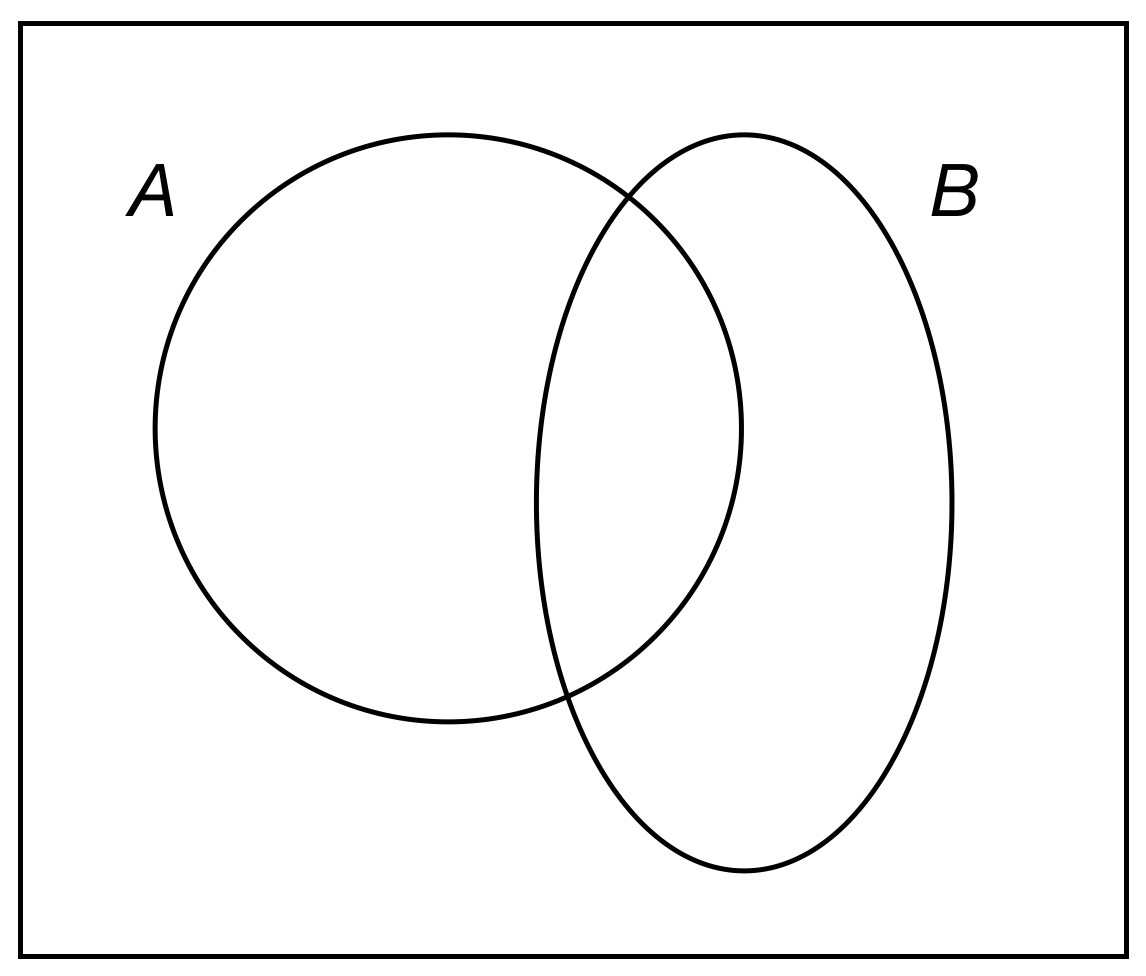
\includegraphics[scale=0.23]{ps2-pic2.png}
\end{center}

\end{itemize}

{\bf Mutual exclusivity:} two events are mutually exclusive or disjoint if they cannot both occur, i.e. 

$$\P(A \cap B) = 0$$ \ 

\begin{itemize}

	\item[8.] What does $\P(A \cup B)$ reduce to if $A$ and $B$ are mutually exclusive? \\ 

	\item[9$i$.] Can you show that $A$ and $B$ cannot be independent if they are mutually exclusive? 
	
\end{itemize}

\hfill 

{\bf Law of total probability:} if the events $B_1, B_2, ..., B_k$ are disjoint and $B_1 \cup B_2 \cup ... \cup B_k = \Omega$ (i.e. they constitute the whole sample space), then for any event $A$:

$$\P(A) = P(A \cap B_1) + \P(A \cap B_2) + ... + \P(A \cap B_k) = \sum_i \P(A \cap B_i) = \sum_i \P(A|B_i)\P(B_i)$$ \ 

This is useful in situations where it's hard to calculate $\P(A)$ by the counting rule but easy to calculate $\P(A|B_i) \P(B_i) ...$.  

\hfill 


\begin{itemize}

	\item[10.] Suppose that half the people on campus get the flu shot. Let $V$ be the event that a person is vaccinated, and $F$ be the event that a person gets the flu, and suppose that $\P(F|V^c) = 0.3$ and $\P(F|V) = 0.1$. What is the probability that a person on campus gets the flu? \\ 
	
	\item[11$i$.] {\it The Monty Hall problem:} You are locked in a room with three doors. Mr. Hall explains to you that behind two of the doors there are mojitos, and behind the third is a mountain lion that will eat you. Mr. Hall instructs you to choose a door and you pick door 1. Mr. Hall then opens door 3, revealing a mojito. Mr. Hall is under oath to open one more door, and offers you the chance to change your pick to door 2. Which door do you instruct Mr. Hall to open in order to minimize your chance of being eaten? Justify your answer.  

\end{itemize}

\hfill 

{\bf Bayes' theorem:} gives the conditional probability of an event, given {\it prior} knowledge related to the event:

$$\P(B|A) = \frac{\P(A|B) \P(B)}{\P(A)} \hspace{1cm} \text{or} \hspace{1cm}\P(B_i|A) = \frac{\P(A|B_i)\P(B_i)}{\sum_j \P(A|B_j)\P(B_j)}$$ \ 

\begin{itemize}

	\item[12$i$.] Three medicines, $A$, $B$, and $C$, can cure ailment in 20\%, 25\%, and 55\% of cases, respectively. However, each medicine causes an adverse side effect in 8\%, 5\%, and 3\% of people, respectively, provided it cures you. Suppose you are blighted by ailment and proceed to take all three medicines. One week later you are cured, but now blighted by the adverse side effect. What is the probability you were cured by medicine $A$, $B$, and $C$, respectively? \\  
		
	\item[13$i$.] In a game of Quidditch, the Snitch is hidden in one of $n$ boxes, and the probability it lies in box $k$ is $P_k$. However, if the Snitch is {\it actually} in box $k$, a search of the box will only reveal it with probability $Q_k$, where $Q_k < P_k$. What is the conditional probability the Snitch is in box $k$ if a search of box $j$ did not reveal it? 

\end{itemize} 





\newpage

{\bf \Large II -- random variables and probability distributions} \\ 

A random variable (RV) assigns a value (usually numeric) to the outcomes of a random process. We usually define the random variable as the quantity we are observing or measuring in an experiment. \\

Random variables are usually denoted by capital letters such as $X$. E.g. if you are observing a coin toss, you could define $X$ as the random variable that it lands heads. For this process $X$ has two possible outcomes, $X=1$ (lands heads) or $X=0$ (lands tails). 

\hfill

\begin{itemize}

	\item[1.] Let $X$ be the random variable for the number of heads you land when tossing a coin 10 times. Open R and simulate this process by running the code $\texttt{sample(x = c(`H',`T'), size = 10, replace = TRUE)}$. This draws a random sample of 10 observations from the sample space ``H" and ``T". Run this process once. What is $X$? Make a frequency table showing the frequency and relative frequency associated with each outcome. Are the results what you expect?  

\end{itemize}

\hfill 

Observing the relative frequency of an event in a number of trials is one way to define the probability of that event---this is known as the {\bfit{frequentist interpretation}} of probability. The frequentist approach assumes that when there are a very large number of trials the observed relative frequency of an event will converge to its true relative frequency (thereby giving a measure of probability). 

\hfill 

\begin{itemize}

	\item[2.] Repeat q1 but with sample sizes $n = \{100, 1000, 100000\}$. Report the relative frequencies of the outcomes for each value of $n$. You may want to use $\texttt{prop.table()}$---see the notes in chapter 7. What do you see?  

\end{itemize}

\hfill

A {\bf probability distribution} describes the probability associated with each value a random variable can take. For discrete RVs, the probability distribution is known as a probability mass function (pmf), as it shows the relative masses or weights of the RV being exactly equal to certain values.   

\hfill 

\begin{itemize}

	\item[3.] Suppose you find yourself in a game of craps, where two six-sided dice are rolled and their face values are added. If the sum is equal to 2, 3, or 12, you lose \$10 times the sum, and if the sum is equal to 7 or 11, you win \$50 times the sum. For any other sum value you lose \$1 (constant). Let $X$ be the RV for your earnings in one such game. Construct a probability distribution (a pmf) for $X$.  

\end{itemize}

\hfill  

The {\bf expected value} of a RV is the average of all possible values it can take, weighted by probability:  

$$\E[X] = \sum_i P_i X_i$$ \ 

Note this is also known as the mean, $\mu$. \\

The {\bf variance} of a RV is the average squared deviation of each value of from the mean, weighted by probability: 

$$\Var[X] = \sum_i  P_i (X_i - \mu)^2 = \E \big[ (X - \mu )^2 \big]$$ \

The variance is also denoted $\sigma^2$. 

\hfill 

\begin{itemize}

	\item[4.] For the distribution in q3, find the expected value and variance. {\it Note:} when computing the variance, you may find it helpful to realize that $\E \big[ (X - \mu )^2 \big] = \E[X^2] - \E[X]^2$. The latter version of the formula will make computations easier. 

\end{itemize}

\hfill 

Note expectation and variance behave slightly differently under linear combinations of random variables. Expectation scales linearly whereas variance does not:

$$\E[2X] = 2 \E[X] \hspace{1cm} \Var[2X] = 2^2 \Var[X]$$ \ 

And while expectation is additive for all RVs, variance is additive only for independent RVs: 

$$\E[X \pm Y] = \E[X] \pm \E[Y] \hspace{1cm} \Var[X \pm Y] = \Var[X] + \Var[Y] \;\;\; \text{(if indep.)}$$ \ 

\begin{itemize}

	\item[5.] Suppose $X$ is the RV for the average economic freedom score in Asia in 2019, and $Y$ is the RV for the equivalent score in 1985. Suppose you know that $\E[X] = 7.6$ and $\Var[X] = 2.3$, and $\E[Y] = 4.2$ and $\Var[Y] = 3.6$. Let $D$ be the RV for the difference in scores between 2019 and 1985. What is the expected value and variance of $D$?  

\end{itemize}





\hfill 

\hfill 

{\bf \Large III -- common probability distributions} \\ 

Below we introduce some known probability distributions that frequently come up in statistical inference. \\ 

The {\bf Bernoulli distribution} can model a discrete random variable with a binary outcome (i.e. success/failure, 1/0, etc.). A single coin toss is an example. The Bernoulli distribution is specified by one parameter, $p$, which describes the probability of a success.  

\hfill 

\begin{itemize}

	\item[1.] Suppose that $X$ is a RV that follows a Bernoulli distribution, i.e. $X \sim \text{Ber}(p)$. Derive expressions for the expected value and variance of $X$. 

\end{itemize}

\hfill 

Let's suppose now that you observe 10 iterations of a Bernoulli process (e.g. 10 coin tosses) and you want to know the probability that exactly four yield successes. How would you calculate this probability? Assuming each trial is independent, you should be able to see that for a given sequence of four successes and six failures the probability is $p^4 (1-p)^6$. Or, more generally, for a given sequence of $n$ trials that comprise $k$ successes, the probability is $p^k (1-p)^{n-k}$. Note however this is the probability of a {\it particular} sequence of successes and failures---to get the {\it total} probability of observing any $k$ successes in $n$ trials, you need to multiply this by the number of ways there are of choosing $k$ items out of $n$. \\ 

{\bfit{A brief detour into combinatorics:}} Consider the number of ways of choosing 2 heads up in a set of 10 coins. You have 10 choices for the first coin, and 9 remaining choices for the second. But you could choose the pair in either order, so the number of {\it distinct} pairs is $\frac{10 \cdot 9}{2}$. To choose 3 coins facing heads up, you have 10 choices for the first, 9 for the second, and 8 for the third. But each triplet has 3 choices for which to flip first, and 2 for which to flip second. So the number of distinct combinations is $\frac{10 \cdot 9 \cdot 8}{3 \cdot 2}$. Following this pattern, the number of distinct ways to choose 4 heads is $\frac{10\cdot 9 \cdot 8 \cdot 7}{4\cdot 3 \cdot 2}$, and the number of distinct ways to choose $k$ heads is $\frac{10 \cdot 9 \cdot ... \cdot (10-k+1)}{k!} = \frac{10!}{k!(10-k)!}$, where $!$ denotes a factorial.  

\hfill 

\begin{itemize}

	\item[2.] Hopefully you see the pattern here. Can you think of a general expression for the number of ways to choose $k$ successes out of $n$ trials?  

\end{itemize}

\hfill 

The expression you just derived is known as the {\bfit{binomial coefficient}}. It forms the basis for the {\bf binomial distribution}, which can model a discrete random variable with a binary outcome over {\it several} trials (e.g. observing several coin tosses). The binomial distribution is specified by two parameters, $n$ (number of trials), and $p$ (probability of a success). For a binomial random variable $X$, its probability distribution is given by:  

$$\text{if} \;\;\; X \sim \text{Bin}(n,p) \hspace{0.5cm} \longrightarrow \hspace{0.5cm} \P(X = k) = \begin{pmatrix} n \\ k \end{pmatrix} p^k (1-p)^{n-k}$$ \ 

where the expression on the right is the pmf of the binomial distribution. Note $\big( \begin{smallmatrix} n \\ k \end{smallmatrix} \big) $ is another way of writing $\frac{n!}{k!(n-k)!}$.  

\hfill 

\begin{itemize}

	\item[3.] How many ways are there of choosing 5 objects out of 10? Use the binomial coefficient explicitly, or use the R function $\texttt{choose(n,k)}$. \\

	\item[4.] For a weighted coin which has a probability of landing heads $p = 0.2$, what is the probability of observing exactly 5 heads in a sequence of 10 tosses? What is the probability of observing at least 2 heads? In R you can compute these using $\texttt{dbinom()}$ and $\texttt{pbinom()}$---but still show your methodology. \\ 

	\item[5.] What conditions must a random process satisfy for the binomial distribution to be a suitable model? \\ 

	\item[6.] Can you derive expressions for the mean and variance of a binomial RV?  

\end{itemize} 

\hfill 

The {\bf normal distribution} (or Gaussian distribution) is one of the most common continuous probability distributions. For a normal random variable $X$, its distribution is symmetric and bell-shaped, given by the following density function: 

$$\text{if} \;\;\; X \sim \mathcal N(\mu,\sigma^2) \hspace{0.5cm} \longrightarrow \hspace{0.5cm} \text{pdf}(X) = \frac{1}{\sqrt{2\pi} \sigma} e^{-(X - \mu)^2/2\sigma^2}$$ \ 

where $\mu$ is the mean and $\sigma^2$ is the variance of the distribution. These two parameters completely specify a normal distribution (increasing $\sigma$ makes it fatter, and changing $\mu$ shifts it left or right).  

\hfill 

\begin{itemize}

	\item[7.] The standard normal distribution has $\mu = 0$ and $\sigma^2 = 1$. Roughly sketch this distribution in the range $\pm 4\sigma$. Remember that $\sim$67\% of values fall within $1\sigma$ of the mean, $\sim$95\% of values fall within $2\sigma$ of the mean, and $\sim$99.5\% of values fall within $3\sigma$ of the mean. \\ 

	\item[8.] Say $X$ is a normally distributed RV with $\mu = 1000$ and $\sigma = 120$. Suppose that on a particular day you observe $X$ and get a value of 1100. The $Z$-score of an observation describes how far away it is from the mean, in units of standard deviation. It is given $Z = \frac{X - \mu}{\sigma}$. What is the $Z$-score of your observed value? \\  

	\item[9.] Suppose you want to determine the probability that on a particular day $X$ is between 800 and 1100, i.e. $\P(800 \leq X \leq 1100)$. To do this: (a) First find the $Z$-score associated with each of the values (b) Next, find the cumulative probability associated with each $Z$-score---you can do this using $Z$-tables, or by using the $\texttt{pnorm()}$ function in R \\ 
(c) Noting that $\P(800 \leq X \leq 1100)$ can also be written $\P(X \leq 1100) - \P(X \leq 800)$, you can simply subtract the two probabilities you found in part (b) to get your answer. \\  

	\item[10.] What is $\P(X \geq 1350)$? What about $\P(X = 1350)$? \\ 

	\item[11.] Suppose you are designing a commercial airplane for 300 passengers. Suppose the weight of every passenger and their belongings is normally distributed with $\mu = 100$ kg and $\sigma = 5$ kg. The airline intends that each plane should fly 100 times per year, and only 15\% of flights should be overweight. Given this information, what total weight should you plan for when designing the plane? \\  

	\item[12$i$.] There are in fact four functions in R that perform probability calculations for normal distributions, $\texttt{qnorm()}$, $\texttt{pnorm()}$, $\texttt{dnorm()}$ and $\texttt{rnorm()}$. There are an equivalent set of functions for the binomial distribution, e.g. $\texttt{qbinom()}$, $\texttt{pbinom()}$, etc. What do each of these functions do? 

\end{itemize}

\hfill

The {\bf Poisson distribution} can model a discrete random variable that tends to occur a fixed number of times during a given interval. It has one parameter, $\lambda$, which describes the average frequency of the event in the interval specified. 

$$\text{if} \;\;\; X \sim \text{Pois}(\lambda) \hspace{0.5cm} \longrightarrow \hspace{0.5cm} \P(X = k) = \frac{\lambda^k e^{-\lambda}}{k!}$$ \ 

\begin{itemize}

	\item[13$i$.] A car dealership sells on average 8 cars per week. What is the probability that during a given month (30 days) it will sell 50 cars? \\  

	\item[14$i$.] {\it The birthday paradox:} What is the probability that two people in a room of $n$ people have the same birthday? Can you show that when $n = 23$ the probability becomes 0.5? \\ 

\end{itemize}












\end{document}
